% !TEX root = ./bursty_transcription.tex
\section{Finding the ``right'' model: Bayesian parameter inference and model 
selection}
\label{section_04_bayesian_inference}
\subsection{Parameter inference for constitutive promoters}

From consideration of Fano factors in the previous section, we suspect that
model 5 in Figure~\ref{fig2:constit_cartoons}(A), a one-state bursty model of
constitutive promoters, achieves a Goldilocks level of complexity. Does this
stand up to closer scrutiny, namely, comparison to full mRNA distributions
rather than simply their moments? We will test this thoroughly on
single-cell mRNA counts for different unregulated promoters from Jones et.\
al.~\cite{Jones2014}.

It will be instructive, however, to first consider the Poisson promoter, model 1
in Figure~\ref{fig2:constit_cartoons}. As we alluded to earlier, since the
Poisson distribution has a Fano factor $\nu$ strictly equal to 1, and all of
the observed data in Figure~\ref{fig2:constit_cartoons}(B) has Fano factor
$\nu>1$, we might already suspect that this model is incapable of fitting the
data. We will verify that this is in fact the case. Using the same argument we
can immediately rule out models 2 and 3 from
Figure~\ref{fig2:constit_cartoons}(A). These models have Fano factors $\nu\le 1$
meaning they are underdispersed relative to the Poisson distribution. We will
also not explicitly consider model 4 from~\fig{fig2:constit_cartoons}(A) since
it was already thoroughly analyzed in~\cite{Razo-Mejia2020}, and since model 5
can be viewed as a special case of it.

Our objective for this section will then be to assess whether or not model 5 is
quantitatively able to reproduce experimental data. In other words, if our claim
is that the level of coarse graining in this model is capable of capturing the
relevant features of the data, then we should be able to find values for the
model parameters that can match theoretical predictions with single-molecule
mRNA count distributions. A natural language for this parameter inference
problem is that of Bayesian probability. We will then build a Bayesian inference
pipeline to fit the model parameters to data. To gain intuition on how this
analysis is done we will begin with the ``wrong'' model 1 in
Figure~\ref{fig2:constit_cartoons}(A). We will use the full dataset of
single-cell mRNA counts from~\cite{Jones2014} used in
Figure~\ref{fig2:constit_cartoons}(B).

\subsubsection{Model 1: Poisson promoter}

For this model the master equation of interest is
Eq.~\ref{eq:poisson_promoter_cme} with repressor set to zero, i.e.,
\begin{equation}
{d\over dt}p_{m,U}(t) = 
        rp_{m-1,U}(t) 
        - rp_{m,U}(t)
        + (m+1)\gamma p_{m+1,U}(t) 
        - \gamma p_{m,U}(t),
\end{equation}
whose steady-state solution is given by a Poisson distribution with parameter
$\lambda \equiv r / \gamma$~\cite{Sanchez2013}. The goal of our inference 
problem is then to find the probability distribution for the parameter value
$\lambda$ given the experimental data. By Bayes theorem this can be written as
\begin{equation}
p(\lambda \mid D) = {p(D \mid \lambda) p(\lambda) \over p(D)},
\end{equation}
where $D = \{m_1, m_2, \ldots, m_N \}$ are the single-cell mRNA experimental
counts. As is standard we will neglected the denominator $p(D)$ on the right
hand side since it is independent of $\lambda$ and serves only as a
normalization factor.

The steady-state solution for the master equation defines the likelihood
term for a single cell $p(m \mid \lambda)$. What this means is that for a given
choice of parameter $\lambda$, under model 1 of
Figure~\ref{fig2:constit_cartoons}(A), we expect to observe $m$ mRNAs in a
single cell with probability
\begin{equation}
p(m\mid\lambda) = \frac{\lambda^m e^{-\lambda}}{m!}.
\label{eq:poisson_inference010}
\end{equation}
Assuming each cell's mRNA count in our dataset is independent of others, the
likelihood of the full inference problem $p(D\mid\lambda)$ is simply a product
of the single cell likelihoods given by \eq{eq:poisson_inference010} above, so
\begin{equation}
p(D\mid\lambda) = \prod_{k=1}^N \frac{\lambda^{m_k}e^{-\lambda}}{m_k!}.
\end{equation}

To proceed we need to specify a prior distribution $p(\lambda)$. In this case we
are extremely data-rich, as the dataset from Jones et.\ al~\cite{Jones2014} has
of order 1000-3000 single-cell measurements for each promoter, so our choice of
prior matters little here, as long as it is sufficiently broad. For details on
the prior selection we refer the reader to Appendix~\ref{sec:bayesian}. For our
purpose here it suffices to specify that we use as prior a Gamma distribution.
This particular choice of prior introduces two new parameters, $\alpha$ and
$\beta$, which parametrize the gamma distribution itself, which we use to encode
the range of $\lambda$ values we view as reasonable. Recall $\lambda$ is the
mean steady-state mRNA count per cell, which \textit{a priori} could plausibly
be anywhere from 0 to a few hundred. $\alpha=1$ and $\beta=1/50$ achieve this,
since the gamma distribution is strictly positive with mean $\alpha/\beta$ and
standard deviation $\sqrt{\alpha}/\beta$.

As detailed in Appendix~\ref{sec:bayesian} this particular choice of prior known
as the \textit{conjugate} prior for a Poisson likelihood. This type of priors
have nice properties to work with, in particular a conjugate prior allows us to
get a closed form for the posterior distribution $p(\lambda \mid D)$. In
particular it can be shown that for a Poisson distribution likelihood with its
Gamma distribution conjugate prior, the posterior distribution is also a Gamma
distribution ~\cite{Gelman2013}. In particular the two parameters $\alpha'$ and
$\beta'$ for this posterior distribution take the form $\alpha' = \alpha +
\bar{m} N$ and $\beta' = \beta + N$, where we defined the sample mean $\bar{m} =
\frac{1}{N}\sum_k m_k$ for notational convenience, and $N$ is the number of
cells n our dataset. Furthermore given that $N$ is $\mathcal{O}(10^3)$ and
$\langle m\rangle \gtrsim 0.1$ for all promoters measured in~\cite{Jones2014}
our data easily overwhelms the choice of prior, and allows us to approximate the
Gamma distribution with a Gaussian distribution with mean $\bar{m}$ and variance
$\bar{m} / N$ with marginal errors. As an example with real numbers, for the
\textit{lacUV5} promoter, Jones et.\ al~\cite{Jones2014} measured 2648 cells
with an average mRNA count per cell of $\bar{m} \approx 18.7$. For this case our
posterior distribution $P(\lambda \mid D)$ would be a Gaussian distribution with
mean $\mu = 18.7$, and a standard deviation $\sigma \approx 0.08$. This suggests
we have inferred our model's one parameter to a precision of order 1\%.

We remind the reader that we began this section claiming that the Poisson model
was ``wrong'' since it could not reproduce features of the data such as a Fano
factor $> 1$. The fact that we got such a narrow posterior distribution for our
parameter $P(\lambda \mid D)$ does not equate to the model being adequate to
describe the data. What this means is that given the data $D$, the parameter 
$\lambda$ for our model is highly constrained to take a narrow range of values,
but a narrow posterior distribution does not speak to the goodness of fit of the
model. As we will see later in Figure~\ref{fig:constit_post_full} after
exploring the bursty promoter model, indeed there is not good correspondence
when contrasting the Poisson model with the experimental .

\subsubsection{Model 5 - Bursty promoter}

Let us now consider the problem of parameter inference for model five
from~\fig{fig1:means_cartoons}(C). As derived in
Appendix~\ref{sec:gen_fcn_appdx}, the steady-state mRNA distribution in this
model is a negative binomial distribution, given by
\begin{equation}
p(m) = \frac{\Gamma(m+k_i)}{\Gamma(m+1)\Gamma(k_i)}
        \left(\frac{1}{1+b}\right)^{k_i}
        \left(\frac{b}{1+b}\right)^m,
\label{eq:neg_bionom}
\end{equation}
where $b$ is the mean burst size and $k_i$ is the burst rate in units of the
mRNA degradation rate $\gamma$. As sketched earlier, to think of the negative
binomial distribution in terms of an intuitive story, we imagine the arrival of
bursts as a Poisson process with rate $k_i$, where each burst has a 
geometrically-distributed size with mean size $b$.

As for the Poisson promoter model, this expression for the steady-state mRNA
distribution is exactly the likelihood we want to use when stating Bayes
theorem. Again denoting the single-cell mRNA count data as $D=\{m_1, m_2,\dots,
m_N\}$, here Bayes theorem takes the form
\begin{equation}
p(k_i, b \mid D) \propto p(D\mid k_i,b)p(k_i, b).
\end{equation}
We already have our likelihood -- the product of $N$ negative binomials as
Eq.~\ref{eq:neg_bionom} -- so we only need to choose priors on $k_i$ and $b$.
For the datasets from~\cite{Jones2014} that we are analyzing, as for the Poisson
promoter model above we are still data-rich so the prior's influence remains
weak, but not nearly as weak because the dimensionality of our model has
increased from one parameter to two. Details on the arguments behind our prior
distribution selection are left for Appendix~\ref{sec:bayesian}. We state here
that the natural scale to explore these parameters is logarithmic. This is
commonly the case for parameters for which our previous knowledge based on our
domain expertise spans several orders of magnitude. For this we chose log-Normal
distributions for both $k_i$ and $b$. Details on the mean and variance of these
distributions can be found in Appendix~\ref{sec:bayesian}.

We carried out MCMC sampling on the posterior of this model, starting with the
constitutive \textit{lacUV5} dataset from~\cite{Jones2014}. The resulting MCMC
samples are shown in Figure~\ref{fig:constit_post_full}(A). In contrast to the
active/inactive constitutive model considered in~\cite{Razo-Mejia2020}
(nonequilibrium model 4 in~\ref{fig2:constit_cartoons}), this model is
well-identified with both parameters determined to a fractional uncertainty of
5-10\%. The strong correlation reflects the fact that their product sets the
mean of the mRNA distribution, which is tightly constrained by the data, but
there is weak ``sloppiness''~\cite{Transtrum2015} along a set of values with a
similar product.

Having found the model's posterior to be well-identified as with the Poisson
promoter, the next step is to compare both models with experimental data. To do
this for the case of the bursty promoter, for each of the parameter samples
shown in Figure~\ref{fig:constit_post_full}(A) we generated negative
bionomial-distributed mRNA counts. As MCMC samples parameter space
proportionally to the posterior distribution, this set of random samples span
the range of possible values that we would expect given the correspondence
between our theoretical model and the experimental data. A similar procedure can
be applied to the Poisson promoter. To compare so many samples with the actual
observed data, we can use empirical cumulative distribution functions (ECDF) of
the distribution quantiles. This representation is shown in
Figure~\ref{fig:constit_post_full}(B). In this example, the median for each
possible mRNA count for the Poisson distribution is shown as a dark green line,
while the lighter green contains 95\% of the randomly generated samples. This
way of representing the fit of the model to the data gives us a sense of the
range of data we might consider plausible, under the assumption that the model
is true. For this case, as we expected given our premise of the Poisson promoter
being wrong, it is quite obvious that the observed data, plotted in black. An 
equivalent plot for the bursty promoter model is shown in blue. Again the darker
tone shows the median, while the lighter color encompasses 95\% of the randomly
generated samples. Unlike the Poisson promoter model, the experimental ECDF
closely tracks the posterior predictive ECDF, indicating this model is actually
able to generate the observed data and increasing our confidence that this model
is at least not wrong.

\textit{lacUV5} is our primary target here, since it forms the core of all the
simple repression constructs of~\cite{Jones2014} that we consider in
Section~\ref{sec:rep_kinetics_inference}. Nevertheless, we thought it wise to
apply our bursty promoter model to the other 17 unregulated promoters available
in the single-cell mRNA count dataset from~\cite{Jones2014} as a test that the
model is capturing the essential phenomenology. If the model fit well to all the
different promoters, this would increase our confidence that it would serve well
as a foundation for inferring repressor kinetics later in
Section~\ref{sec:rep_kinetics_inference}. Conversely, were the model to fail on
more than a couple of the other promoters, it would give us pause.

\begin{figure}%[h!]
\centering
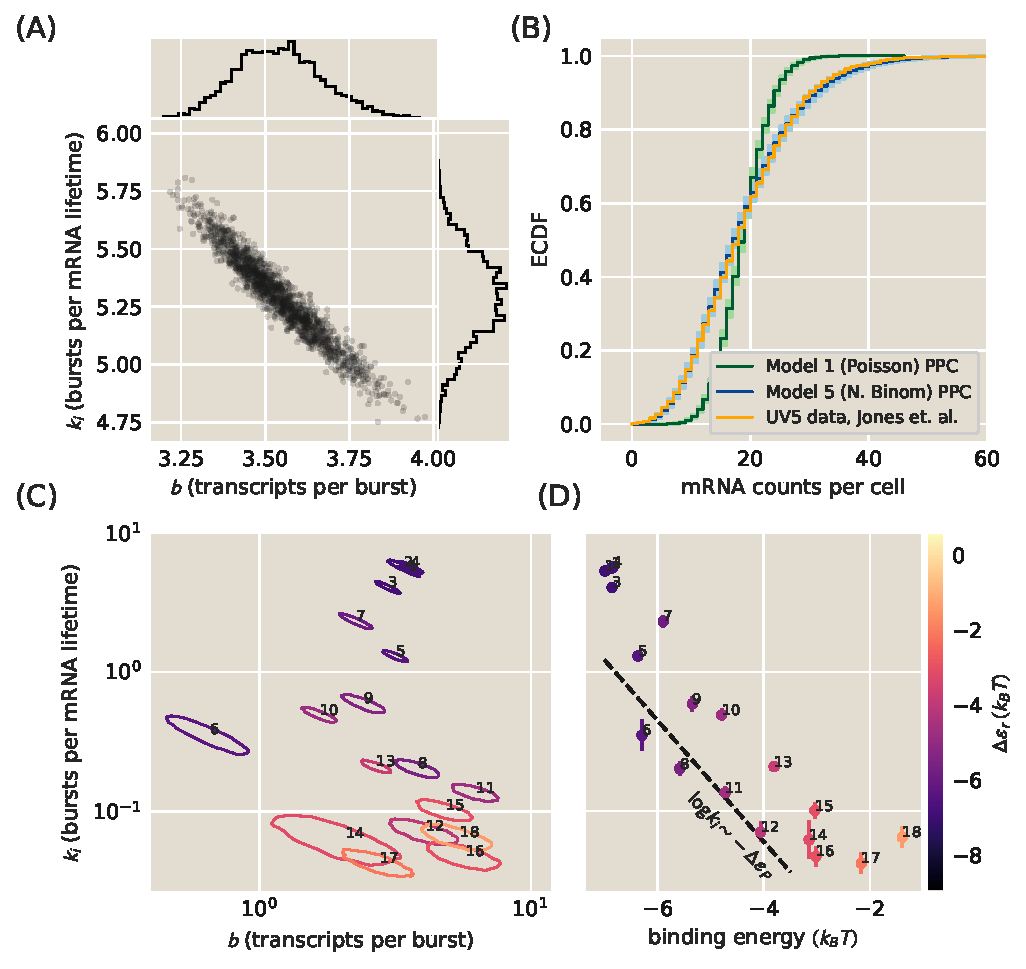
\includegraphics[width=\textwidth]{../figures/main/fig03.pdf}
\caption{\textbf{Constitutive promoter posterior inference and model
comparison.} (A) The joint posterior density of model 5, the bursty promoter
with negative binomially-distributed steady state, is plotted with MCMC samples.
1D marginal probability densities are plotted as flanking histograms. The model
was fit on \textit{lacUV5} data from~\cite{Jones2014}. (B) The empirical
distribution function (ECDF) of the observed population distribution of mRNA
transcripts under the control of a constitutive \textit{lacUV5} promoter is
shown in orange. The median posterior predictive ECDFs for models (1), Poisson,
and (5), negative binomial, are plotted in dark green and dark blue,
respectively. Lighter green and blue regions enclose 95\% of all posterior
predictive samples from their respective models. Model (1) is in obvious
contradiction with the data while model (5) is not. Single-cell mRNA count data
is again from~\cite{Jones2014}. (C) Joint posterior distributions for burst rate
$k_i$ and mean burst size $b$ for 18 unregulated promoters
from~\cite{Jones2014}. Each contour indicates the 95\% highest posterior
probability density region for a particular promoter. Note that the vertical
axis is shared with (D). (D) Plots of the burst rate $k_i$ vs.\ the binding
energy for each promoter as predicted in~\cite{Brewster2012}. The dotted line
shows the predicted slope according to Eq.~\ref{eq:bursty_equil_corresp1},
described in text. Each individual promoter is labeled with a unique number in
both (C) and (D) for cross comparison and for comparison with 
Figure~\ref{fig2:constit_cartoons}(B).}
\label{fig:constit_post_full}
\end{figure}

\fig{fig:constit_post_full}(C) shows the results, plotting the posterior
distribution from individually MCMC sampling all 18 constitutive promoter
datasets from~\cite{Jones2014}. To aid visualization, rather than plotting
samples for each promoter's posterior as in \fig{fig:constit_post_full}(A), for
each posterior we find and plot the curve that surrounds the 95\% highest
probability density region. What this means is that each contour 
encloses approximately 95\% of the samples, and thus 95\% of the probability
mass, of its posterior distribution. Theory-experiment comparisons (not shown)
display a similar level of agreement between data and predictive samples as for
the bursty model with \textit{lacUV5} in \fig{fig:constit_post_full}(B).
\mmnote{Might be worth showing some/all of these PPCs in supplement for
completeness? We could do postage stamp sized diff plots and probably fit all 18
promoters on 1-2 pages.}\mrm{Definitely need to show them in SI.}

One interesting feature from \fig{fig:constit_post_full}(C) is that burst rate
varies far more widely, over a range of $\sim10^2$, than burst size, confined to
a range of $\lesssim10^1$ (and with the exception of promoter 6, just a span of
3-5x). This suggests that $k_i$, not $b$, is the key dynamic variable that
promoter sequence tunes.

It is interesting to connect this observation to the work
of~\cite{Brewster2012}, where these same 18 promoters were considered through
the lens of the three-state equilibrium model (model 2 in
Figure~\ref{fig1:means_cartoons}(B)) and binding energies $\Delta\varepsilon_P$
were predicted from an energy matrix model derived from~\cite{Kinney2010}. As
previously discussed the thermodynamic models of gene regulation can only make
statements about the mean gene expression. This implies that we can draw the
connection between both frameworks by equating the mean mRNA $\left\langle m
\right\rangle$. This results in
\begin{equation}
\langle m \rangle = \frac{k_i b}{\gamma}
        = \frac{r}{\gamma}
        \frac{\frac{P}{N_{NS}}\exp(-\beta\Delta\varepsilon_P)}
                {1+\frac{P}{N_{NS}}\exp(-\beta\Delta\varepsilon_P)}.
\end{equation}
By taking the weak promoter approximation for the equilibrium model ($P/N_{NS} 
\exp(-\beta\Delta\varepsilon_r) \ll 1$) results in
\begin{equation}
\langle m \rangle = \frac{k_i b}{\gamma}
        = \frac{r}{\gamma} \frac{P}{N_{NS}}\exp(-\beta\Delta\varepsilon_P),
\end{equation}
valid for all the binding energies considered here.

Given this result, how are the two coarse-grainings related? A quick estimate
can shed some light. Consider for instance the \textit{lacUV5} promoter, which
we see from Figure~\ref{fig:constit_post_full}(A) has $k_i/\gamma \sim b \sim
\text{few}$, from Figure~\ref{fig:constit_post_full}(B) has $\langle m \rangle
\sim 20$, and from~\cite{Brewster2012} has $\beta\Delta\epsilon_P \sim - 6.5$.
Further we generally assume $P/N_{NS} \sim 10^{-3}$ since
$N_{NS}\approx4.6\times10^6$ and $P\sim10^3$. After some guess-and-check with
these values, one finds the only association that makes dimensional sense and
produces the correct order-of-magnitude for the known parameters is to take
\begin{equation}
\frac{k_i}{\gamma} = \frac{P}{N_{NS}} \exp(-\beta\Delta\varepsilon_P)
\label{eq:bursty_equil_corresp1}
\end{equation}
and
\begin{equation}
b = \frac{r}{\gamma}.
\label{eq:bursty_equil_corresp2}
\end{equation}
Figure~\ref{fig:constit_post_full}(D) shows that this linear scaling between
$\ln k_i$ and $-\beta\Delta\varepsilon_P$ is approximately true for all 18
constitutive promoters considered. The plotted line is simply
Eq.~\ref{eq:bursty_equil_corresp1} and assumes $P\approx 5000$.

While the associations represented by Eq.~\ref{eq:bursty_equil_corresp1} and
Eq.~\ref{eq:bursty_equil_corresp2} appear to be born out by the data in
Figure~\ref{fig:constit_post_full}, we do not find the association of parameters
they imply to be intuitive. We are also cautious to ascribe too much physical
reality to the parameters. Indeed, part of our point in comparing the various
constitutive promoter models is to demonstrate that these models each provide an
internally self-consistent framework that adequately describes the data, but
attempting to translate between models reveals the dubious physical
interpretation of their parameters.

\mmnote{Outline, still to cover:
\begin{itemize}
\item There is a puzzle in comparing w/ Chong2014 supercoiling
model: if supercoiling is the thing, why are my burst sizes all
the same but burst rates vary? And why is the duty cycle of my
promoter so low, ie., bursts so short? COmpare their fig 7E;
their $\beta/\alpha$ is my $k^+/k^-$. They have one or two genes
with very small $\beta/\alpha$, does the \textit{galK} locus just
happen to be that, or is there a deeper disagreement? Hard to say
w/o more data. Are we
missing important things?? Unclear, we leave as open question. Good enough for
our purposes: posterior is identifiable, PPC is great, and of the models we've
thought of it is unique in satisfying both.
\end{itemize}
}

\subsection{Transcription factor kinetics can be inferred from FISH
measurements}\label{sec:rep_kinetics_inference}

Now that we have a satisfactory model in hand for constitutive promoters, we
would like to return to the main thread: can we infer repressor binding and
unbinding rates from mRNA distributions over a population of cells as measured
by single-molecule FISH in~\cite{Jones2014}? If so, how do these inferred rates
compare to direct single-molecule measurements such as from~\cite{Hammar2014}
and to binding energies such as from~\cite{Garcia2011a}
and~\cite{Razo-Mejia2018}, which were inferred under the assumptions of the
equilibrium models in Figure~\ref{fig1:means_cartoons}(B)? And can this
comparison shed light on the unreasonable effectiveness of the equilibrium
models?

\begin{figure}%[h!]
\centering
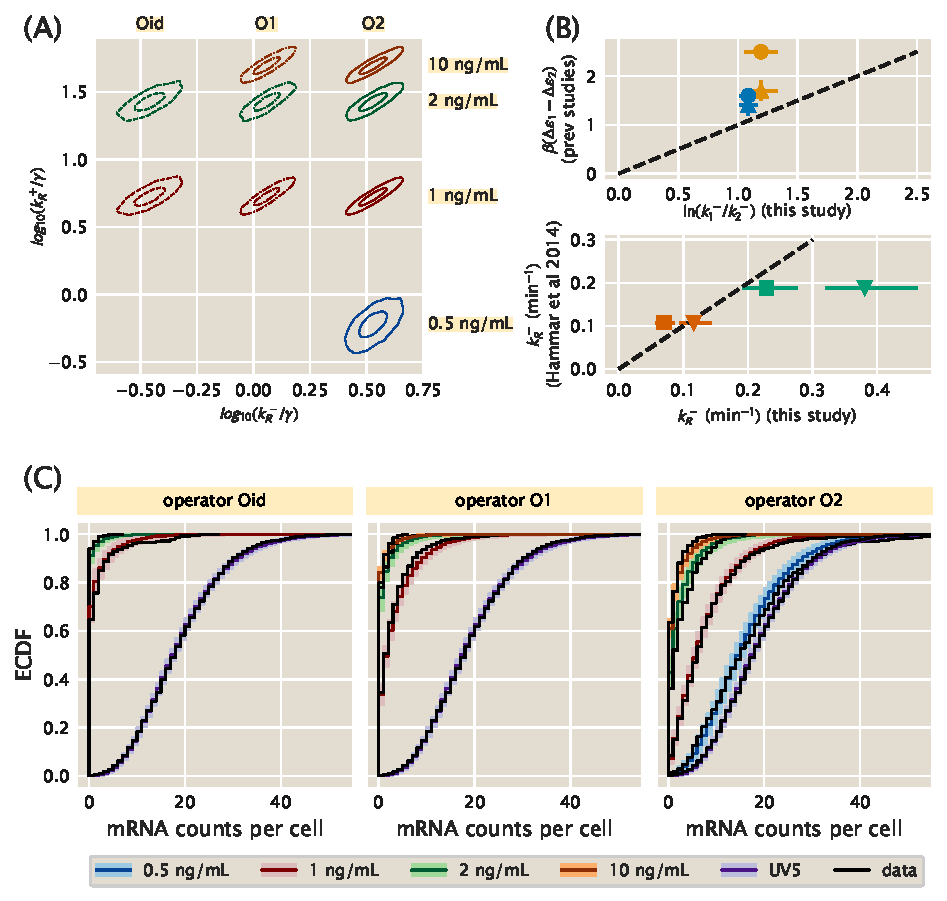
\includegraphics[width=\textwidth]{../figures/main/fig04.pdf}
\caption{\textbf{Simple repression parameter inference and comparison.}
(A) Contours which enclose 50\% and 95\% of the posterior probability mass are
shown for each of several 2D slices of the 9D posterior distribution. The model
assumes one unbinding rate for each operator (Oid, O1, O2) and one binding rate
for each aTc induction concentration (corresponding to an unknown mean repressor
copy number). (B, upper panel) Ratios of our inferred unbinding rates are
compared with operator binding energy differences measured by Garcia and
Phillips~\cite{Garcia2011a} (triangles) and Razo-Mejia et.\
al.~\cite{Razo-Mejia2018} (circles). Blue glyphs compare O2-O1, while orange
compare O1-Oid. (B, lower panel) Unbinding rates for O1 (cyan) and Oid (red)
inferred in this work are compared with single-molecule measurements of the same
from Hammar et.\ at.\ 2014. The comparison requires an assumption about mRNA
lifetime $\gamma^{-1}$, which was not measured, and we plot representative
choices assuming $\gamma^{-1}=3$~min (triangles) or $\gamma^{-1}=5$~min
(squares). (C) Theory-experiment comparison are shown for each of the datasets
used in the inference of the model in (A). Observed single-molecule mRNA counts
data from~\cite{Jones2014} is plotted as black lines. The median of the randomly
generated samples for each condition is plotted as a dark colored line. Lighter
colored bands enclose 95\% of all samples for a given operator/repressor copy
number pair. Samples are sorted by operator and plotted separately for visual
clarity. The unregulated promoter, UV5, is shown with each as a reference
point.}
\label{fig4:repressed_post_full}
\end{figure}

As we found in Section~\ref{sec:beyond_means}, for our purposes the ``right''
model of a constitutive promoter is the bursty picture, model five in
Figure~\ref{fig2:constit_cartoons}. Therefore our starting point here is the
analogous model with repressor added, model 5 in
Figure~\ref{fig1:means_cartoons}(C). For a given repressor binding site and copy
number, this model has four rate parameters to be inferred: the repressor
binding and unbinding rates $k_R^+$, and $k_R^-$, the initiation rate of bursts,
$k_i$, and the mean burst size $b$ (we nondimensionalize all of these by the
mRNA degradation rate $\gamma$).

Before showing the mathematical formulation of our statistical inference model,
we would like to sketch the intuitive structure. The dataset
from~\cite{Jones2014} we consider consists of single-cell mRNA FISH measurements
of nine different conditions, spanning several combinations of three unique
repressor binding sites and four unique repressor copy numbers. We assume that
the values of $k_i$ and $b$ are known, since we have already cleanly inferred
them from constitutive promoter data, and further we assume that these values
are the same across datasets with different repressor binding sites and copy
numbers. In other words, we assume that the regulation of the transcription
factor does not affect the mean burst size nor the burst initiation rate. The
regulation happens as the promoter is taken away from the transcriptionally
active state when the promoter is bound. We assume that there is one unbinding
rate parameter for each repressor binding site, which is shared across aTc
inducer conditions, and likewise one binding rate for each unique repressor copy
number. This makes our model nine dimensional, or nine if one counts $k_i$ and
$b$ as well.

Formally now, denote the set of seven repressor rates to be inferred as
\begin{equation}
\vect{k} =\{k_{Oid}^-, k_{O1}^-, k_{O2}^-,
k_{0.5}^+, k_{1}^+, k_{2}^+, k_{10}^+\},
\end{equation}
where subscripts for dissociation rates $k^-$  indicate the different repressor
binding sites, and subscripts for association rates $k^+$ indicate the aTc
concentration at which the repressor itself was induced. We emphasize that for
this particular dataset the repressor copy numbers are not known directly, so we
label their association rates by the concentration of a small molecule inducer
aTc which indirectly controls the transcription of $\textit{lacI}$. Also note
that the authors of~\cite{Jones2014} report estimates of LacI copy number per
cell rather than direct measurements. However, these estimates were made
\textit{assuming} the validity of the equilibrium models in
Figure~\ref{fig1:means_cartoons}, and since \textit{testing} these models is our
goal, we will make no assumptions about the LacI copy number for given aTc
concentrations.

Having stated the problem, Bayes theorem reads simply
\begin{equation}
p(\vect{k}, k_i, b \mid D)
\propto
p(D \mid\vect{k}, k_i, b) p(\vect{k}, k_i, b),
\end{equation}
where $D$ is again the set of all $N$ observed single-cell mRNA counts
across the various conditions. We assume that individual single-cell
measurements are independent so that the likelihood factorizes as
\begin{equation}
p(D \mid\vect{k}, k_i, b)
= \prod_{j=1}^N p(m\mid \vect{k}, k_i, b)
= \prod_{j=1}^N p(m\mid k_j^+, k_j^-, k_i, b)
\end{equation}
where $k_j^\pm$ represent the appropriate binding and unbinding
rates out of $\vect{k}$ for the $j$-th measured cell. The probability
$p(m\mid k_j^+, k_j^-, k_i, b)$ appearing in the last expression
is exactly Eq.~\ref{eq:p_m_bursty+rep_appdx}, the steady-state
distribution for our bursty model with repression derived in
Section~\ref{sec:gen_fcn_appdx}, which for completeness we reproduce here as
\begin{equation}
\begin{split}
p(m \mid k_R^+, k_R^-, k_i, b) = & ~\frac{
        \Gamma(\alpha + m)\Gamma(\beta + m)\Gamma(k_R^+ + k_R^-)
        }
        {
        \Gamma(\alpha)\Gamma(\beta)\Gamma(k_R^+ + k_R^- + m)
        }
\frac{b^m}{m!}
\\
&\times {_2F_1}(\alpha+m, \beta+m, k_R^++k_R^-+m; -b).
\end{split}
\label{eq:p_m_bursty+rep}
\end{equation}
where $\alpha$ and $\beta$, defined for notational convenience, are
\begin{align}
\begin{split}
\alpha &= \frac{1}{2}
\left(k_i+k_R^-+k_R^+ + \sqrt{(k_i+k_R^-+k_R^+)^2 - 4k_i k_R^-}\right)
\\
\beta &= \frac{1}{2}
\left(k_i+k_R^-+k_R^+ - \sqrt{(k_i+k_R^-+k_R^+)^2 - 4k_i k_R^-}\right).
\end{split}
\end{align}

\mmnote{Probably SI most of this paragraph?}
This likelihood is rather inscrutable. We did not find any of the known
analytical approximations for ${_2F_1}$ terribly useful in gaining intuition, so
we instead resorted to numerics. One insight we found
\mmnote{a plot would probably help explain, maybe SI, need to explain better}
was that for very strong or very weak repression, the distribution in
Eq.~\ref{eq:p_m_bursty+rep} is well approximated by a negative binomial with
burst size $b$ and burst rate $k_i$ equal to their constitutive \textit{lacUV5}
values, except with $k_i$ multiplied by the fold-change
$\left(1+k_R^+/k_R^-\right)^{-1}$. In other words, once again only the
\textit{ratio} $k_R^+/k_R^-$ was detectable. But for intermediate repression,
the distribution was visibly broadened with Fano factor greater than $1+b$, the
value for the corresponding constitutive case. This indicates that the repressor
rates had left an imprint on the distribution, and perhaps intuitively, this
intermediate regime occurs for values of $k_R^\pm$ comparable to the burst rate
$k_i$. Put another way, if the repressor rates are much faster or much slower
than $k_i$, then there is a timescale separation and effectively only one
timescale remains, $k_i\left(1+k_R^+/k_R^-\right)^{-1}$. Only when all three
rates in the problem are comparable does the mRNA distribution retain detectable
information about them.

Next we specify priors. As for the constitutive model, weakly informative
lognormal priors are a natural choice for all our rates. We found that if the
priors were too weak, our MCMC sampler would often become stuck in regions of
parameter space with very low probability density, unable to move. We struck a
balance in choosing our prior widths between helping the sampler run while
simultaneously verifying that the marginal posteriors for each parameter were
not artificially constrained or distorted by the presence of the prior. The only
exception to this is the highly informative priors we placed on $k_i$ and $b$,
since we have strong knowledge of them from our inference of constitutive
promoters above. All details for our prior distributions are listed in 
Appendix~\ref{sec:bayes}.

We ran MCMC sampling on the full nine dimensional posterior specified by this
generative model. To attempt to visualize this object, in
Figure~\ref{fig4:repressed_post_full}(A) we plot several two-dimensional slices
as contour plots, analogous to Figure~\ref{fig:constit_post_full}(C). Each of
these nine slices corresponds to the $(k_R^+, k_R^-)$ pair of rates for one of
the conditions from the dataset used to fit the model and gives a
sense of the uncertainty and correlations in the posterior.
\mrm{before invoking part (C) of the figure we are missing th explanation for 
part (B). I don't fully understand how these computations were made, so I'll 
let Jupiter detail this.}

% With priors and likelihood specified we may write down our complete generative model as
% \begin{equation}
% \begin{split}
% \log_{10}k_i &\sim \text{Normal}(0.725, 0.025)\\
% \log_{10}b   &\sim \text{Normal}(0.55, 0.025)\\
% \log_{10}k_{0.5}^+ &\sim \text{Normal}(-0.45, 0.3)\\
% \log_{10}k_{1}^+   &\sim \text{Normal}(0.6, 0.3)\\
% \log_{10}k_{2}^+   &\sim \text{Normal}(1.15, 0.3)\\
% \log_{10}k_{10}^+  &\sim \text{Normal}(1.5, 0.3)\\
% \log_{10}k_{Oid}^- &\sim \text{Normal}(-0.25, 0.3)\\
% \log_{10}k_{O1}^-  &\sim \text{Normal}(0.1, 0.3)\\
% \log_{10}k_{O2}^-  &\sim \text{Normal}(0.45, 0.3)\\
% m &\sim \text{Likelihood}(k_R^+, k_R^-, k_i, b),
% \end{split}
% \end{equation}
% where the likelihood is specified by Eq.~\ref{eq:p_m_bursty+rep}.
% \mmnote{Now that I've typed this out, this notation seems totally
% pointless here, especially when the likelihood is not a standard
% distribution. Maybe I should make a table or something to record
% the prior values, and maybe even that should go to SI?}

